\documentclass[8pt]{article}

\usepackage{arxiv}
\usepackage[utf8]{inputenc}    % allow utf-8 input
\usepackage[T1]{fontenc}       % use 8-bit T1 fonts
\usepackage{hyperref}          % hyperlinks
\usepackage{url}               % simple URL typesetting
\usepackage{booktabs}          % professional-quality tables
\usepackage{amsfonts}          % blackboard math symbols
\usepackage{nicefrac}          % compact symbols for 1/2, etc.
\usepackage{microtype}         % microtypography
\usepackage{graphicx}
\usepackage{natbib}
\usepackage{doi}
\usepackage{amsmath}           % for math environments if needed
\usepackage{xcolor}            % for coloring text
\usepackage[inline]{enumitem}  % for listing horizontally
\usepackage{minted}            % for code

\parskip 4.2pt  % Sets spacing between paragraphs.

% Minted configuration
\usemintedstyle{default}
\renewcommand{\theFancyVerbLine}{\sffamily \arabic{FancyVerbLine}}
\floatstyle{plaintop}
\newfloat{program}{thp}{lop}
\floatname{program}{program}

\definecolor{LightGray}{gray}{0.9}

\setminted{
  tabsize=8,
  frame=lines,
  framesep=2mm,
  baselinestretch=1.2,
  bgcolor=LightGray,
  fontsize=\footnotesize,
}
% End minted configuration

\title{Risk Analysis and Pricing in Non-Life Insurance}

% Optionally, you can include date or leave it blank:
\date{\today}


\author{%
  Björn Thor Stefánsson \\
  University of Iceland \\
  \texttt{bts5@hi.is}
  \And
  Viktor Már Guðmundsson \\
  University of Iceland \\
  \texttt{vmg3@hi.is} 
  %% More authors can be added here
}

% Uncomment to remove the date
\date{April 15, 2025}

% Uncomment to override the default 'A preprint' in the header
\renewcommand{\headeright}{Final Project}
\renewcommand{\undertitle}{Non-Life Insurance Mathematics}
\renewcommand{\shorttitle}{Risk Analysis and Pricing} % Need new name

\hypersetup{
  pdftitle={Risk Analysis and Pricing in Non-Life Insurance},
  pdfsubject={Non-Life Insurance, Premiums, Pricing, Large Claims},
  pdfauthor={Björn Thor Stefánsson, Viktor Már Guðmundsson},
  pdfkeywords={Non-Life Insurance, Premiums, Pricing, Large Claims},
}

\begin{document}
\maketitle

\begin{abstract}
  This report analyzes pricing strategies and risk assessment methods in non-life insurance. We explore pure premium estimation using actuarial models and examine the impact of reinsurance on large claims through simulation-based techniques. The findings provide insights into optimal pricing strategies and financial risk mitigation.
\end{abstract}

% keywords can be removed
\keywords{Non-Life Insurance \and Premium Estimation \and Large Claim Analysis}

\section{Introduction}
% Brief context for both Part A and Part B
\label{sec:intro}
Accurate risk assessment and pricing are essential in non-life insurance to ensure financial stability and competitiveness. Insurers must balance fair premium pricing with profitability while managing uncertainty in claim costs. 

This report focuses on two key aspects of risk analysis. First, we estimate pure premiums using actuarial models to identify risk factors and optimize pricing strategies. Second, we analyze large claims and evaluate the impact of reinsurance contracts on financial performance. By leveraging statistical modeling and simulation techniques, we provide insights that support data-driven decision-making in insurance pricing and risk mitigation.

\section{Pure Premium Estimation and Risk-Based Pricing}
\label{sec:partA}

Example

In this part, we created DDPMs based on the architecture proposed by \href{https://arxiv.org/abs/2006.11239}{Ho et al, 2020,} for generating 28x28 greyscale images of handwritten digits from 0 to 9 using the MNIST dataset. We started with the simple diffusion model from the {\color{blue}\small{\texttt{mnist\_ddpm\_solutions.ipynb}}} notebook and extended it with 4 variants. We compare the models' performance visually and quantitatively. The visual plots are in Appendix

\subsection{Data Exploration and Preprocessing}
% Overview of dataset structure and key variables.
% Handling missing data and potential outliers.

\subsection{Model Selection and Implementation}
	% •	Justification for using Generalized Linear Models (GLMs).
	% •	Model specifications and variable selection.
	% •	Training methodology and hyperparameter tuning.

\subsection{Risk Segmentation and Pricing Adjustments}
	% •	Identifying high-risk and low-risk policyholders.
	% •	Calculating risk-adjusted premiums.
	% •	Impact of different pricing strategies.


\subsection{Model Evaluation and Performance Metrics}
	% •	Loss functions and model validation methods.
	% •	Comparing predicted vs. actual claim frequencies.
	% •	Business implications of model accuracy.

\newpage

\section{Large Claim Analysis and Reinsurance Impact (Skoða áhrif tíma?)}
\label{sec:partB}
% (Uppfæra 3.5 tengja við quantiles í 3.4) og nota vigtaða summu tveggja dreifinga fyrir tjónin (stór og lítil) Ættum að skoða hvort tími hefur einhver áhrif eða ártalið
% Var ekki einhver regla sem segir til hvort fyrirtækið verði gjaldþrota eða ekki? Það var tengt jákvæðum hleðslum í iðgjöldum
% Og önnur regla fyrir modeling á svona distribution ein dreifing fyrir non extreme og sér dreifing fyrir extreme? Það er parametric leið en MCMC er non parametric


A Danish insurance company has collected data on fire damage claims from 2010 to 2020. The claims are measured in millions of Danish kroner (DKK). The company has $630\,000$ fire insurance policies, with an annual claim frequency of 900 per million policies. The current premium per policy is $3\,331$ DKK.

The company is evaluating two Excess-of-Loss (XL) reinsurance contracts:
\begin{enumerate}
    \item[1.] \textbf{Contract 1:} The insurer retains up to 10 million DKK per claim, and the reinsurer covers excess losses up to 40 million DKK. The reinsurance premium is 609 DKK per policy.
    \item[2.] \textbf{Contract 2:} The insurer retains 10 million DKK, and the reinsurer covers all excess losses without an upper limit. The reinsurance premium is 872 DKK per policy.
\end{enumerate}


\subsection{Loss Distribution Analysis}
To assess the risk profile of the insurance portfolio, we analyze the severity distribution of claims. The dataset reveals a heavy-tailed loss distribution, indicating a small number of high-cost claims.

\begin{figure}[h]
    \centering
    \begin{minipage}{0.48\textwidth}
        \centering
        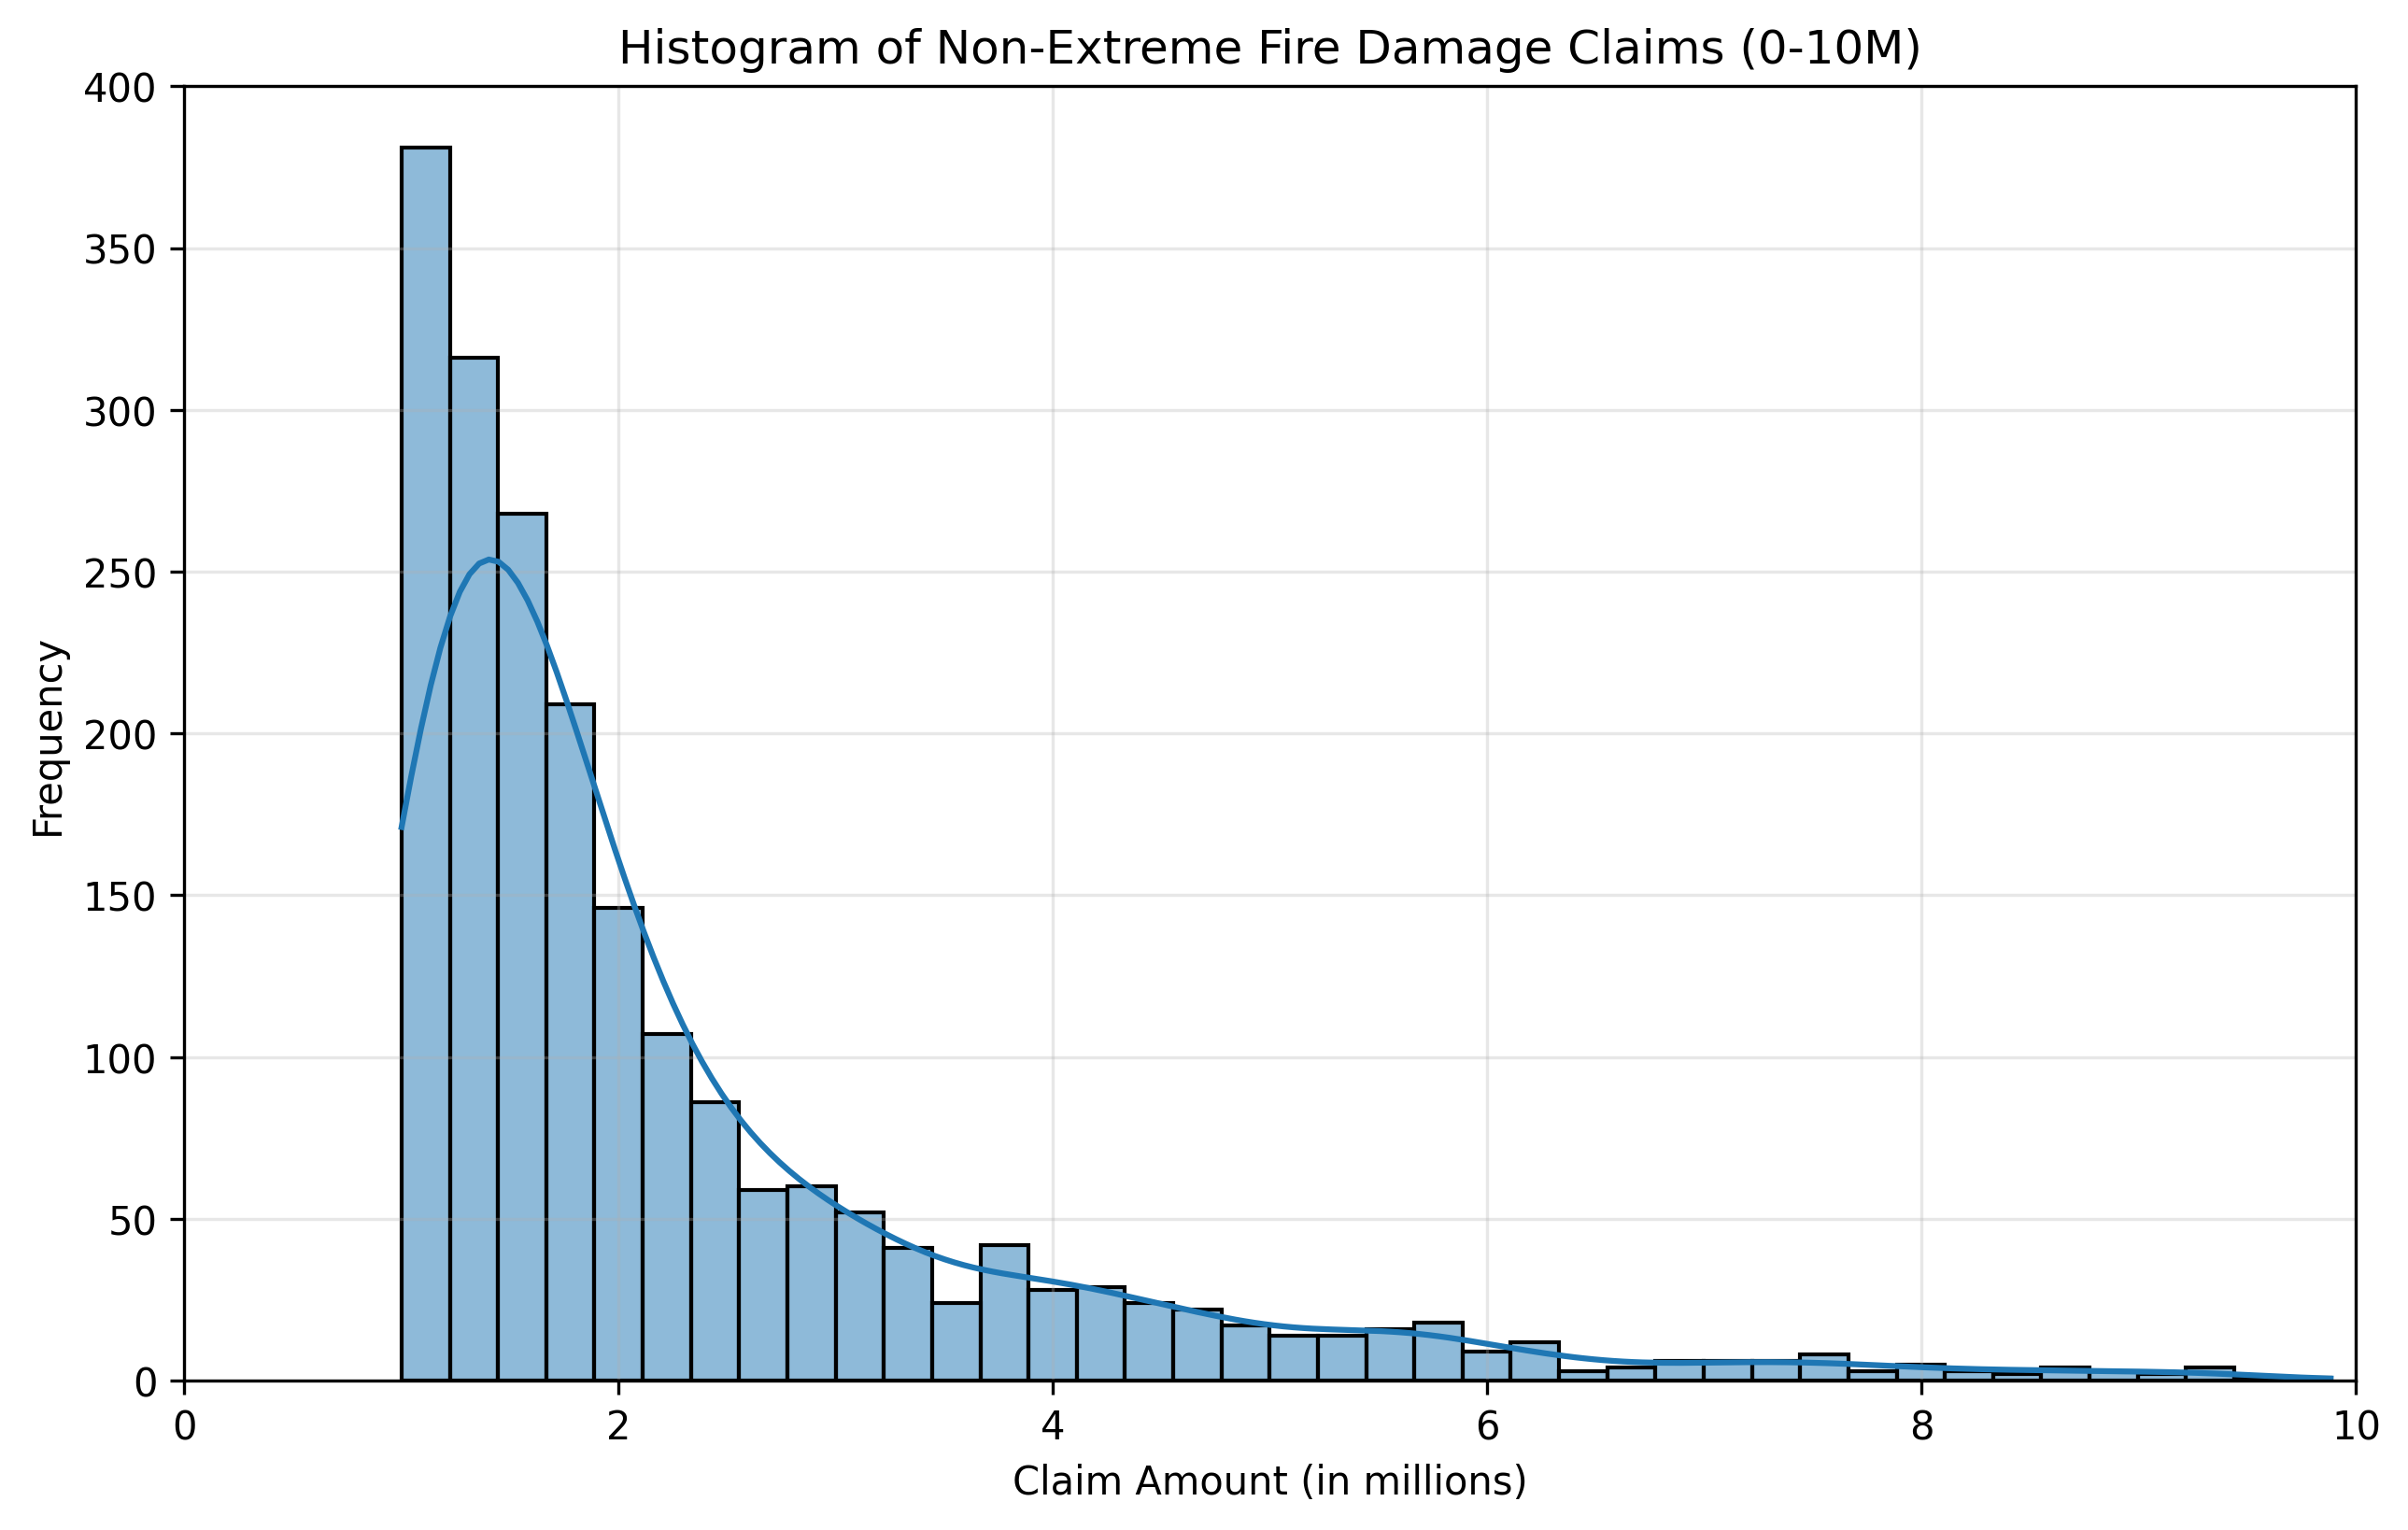
\includegraphics[width=\linewidth]{Figures/histogram_normal.png}
        \caption{Non-Extreme Fire Damage Claims ($\leq10$M)}
        \label{fig:histo-normal}
    \end{minipage}
    \hfill
    \begin{minipage}{0.48\textwidth}
        \centering
        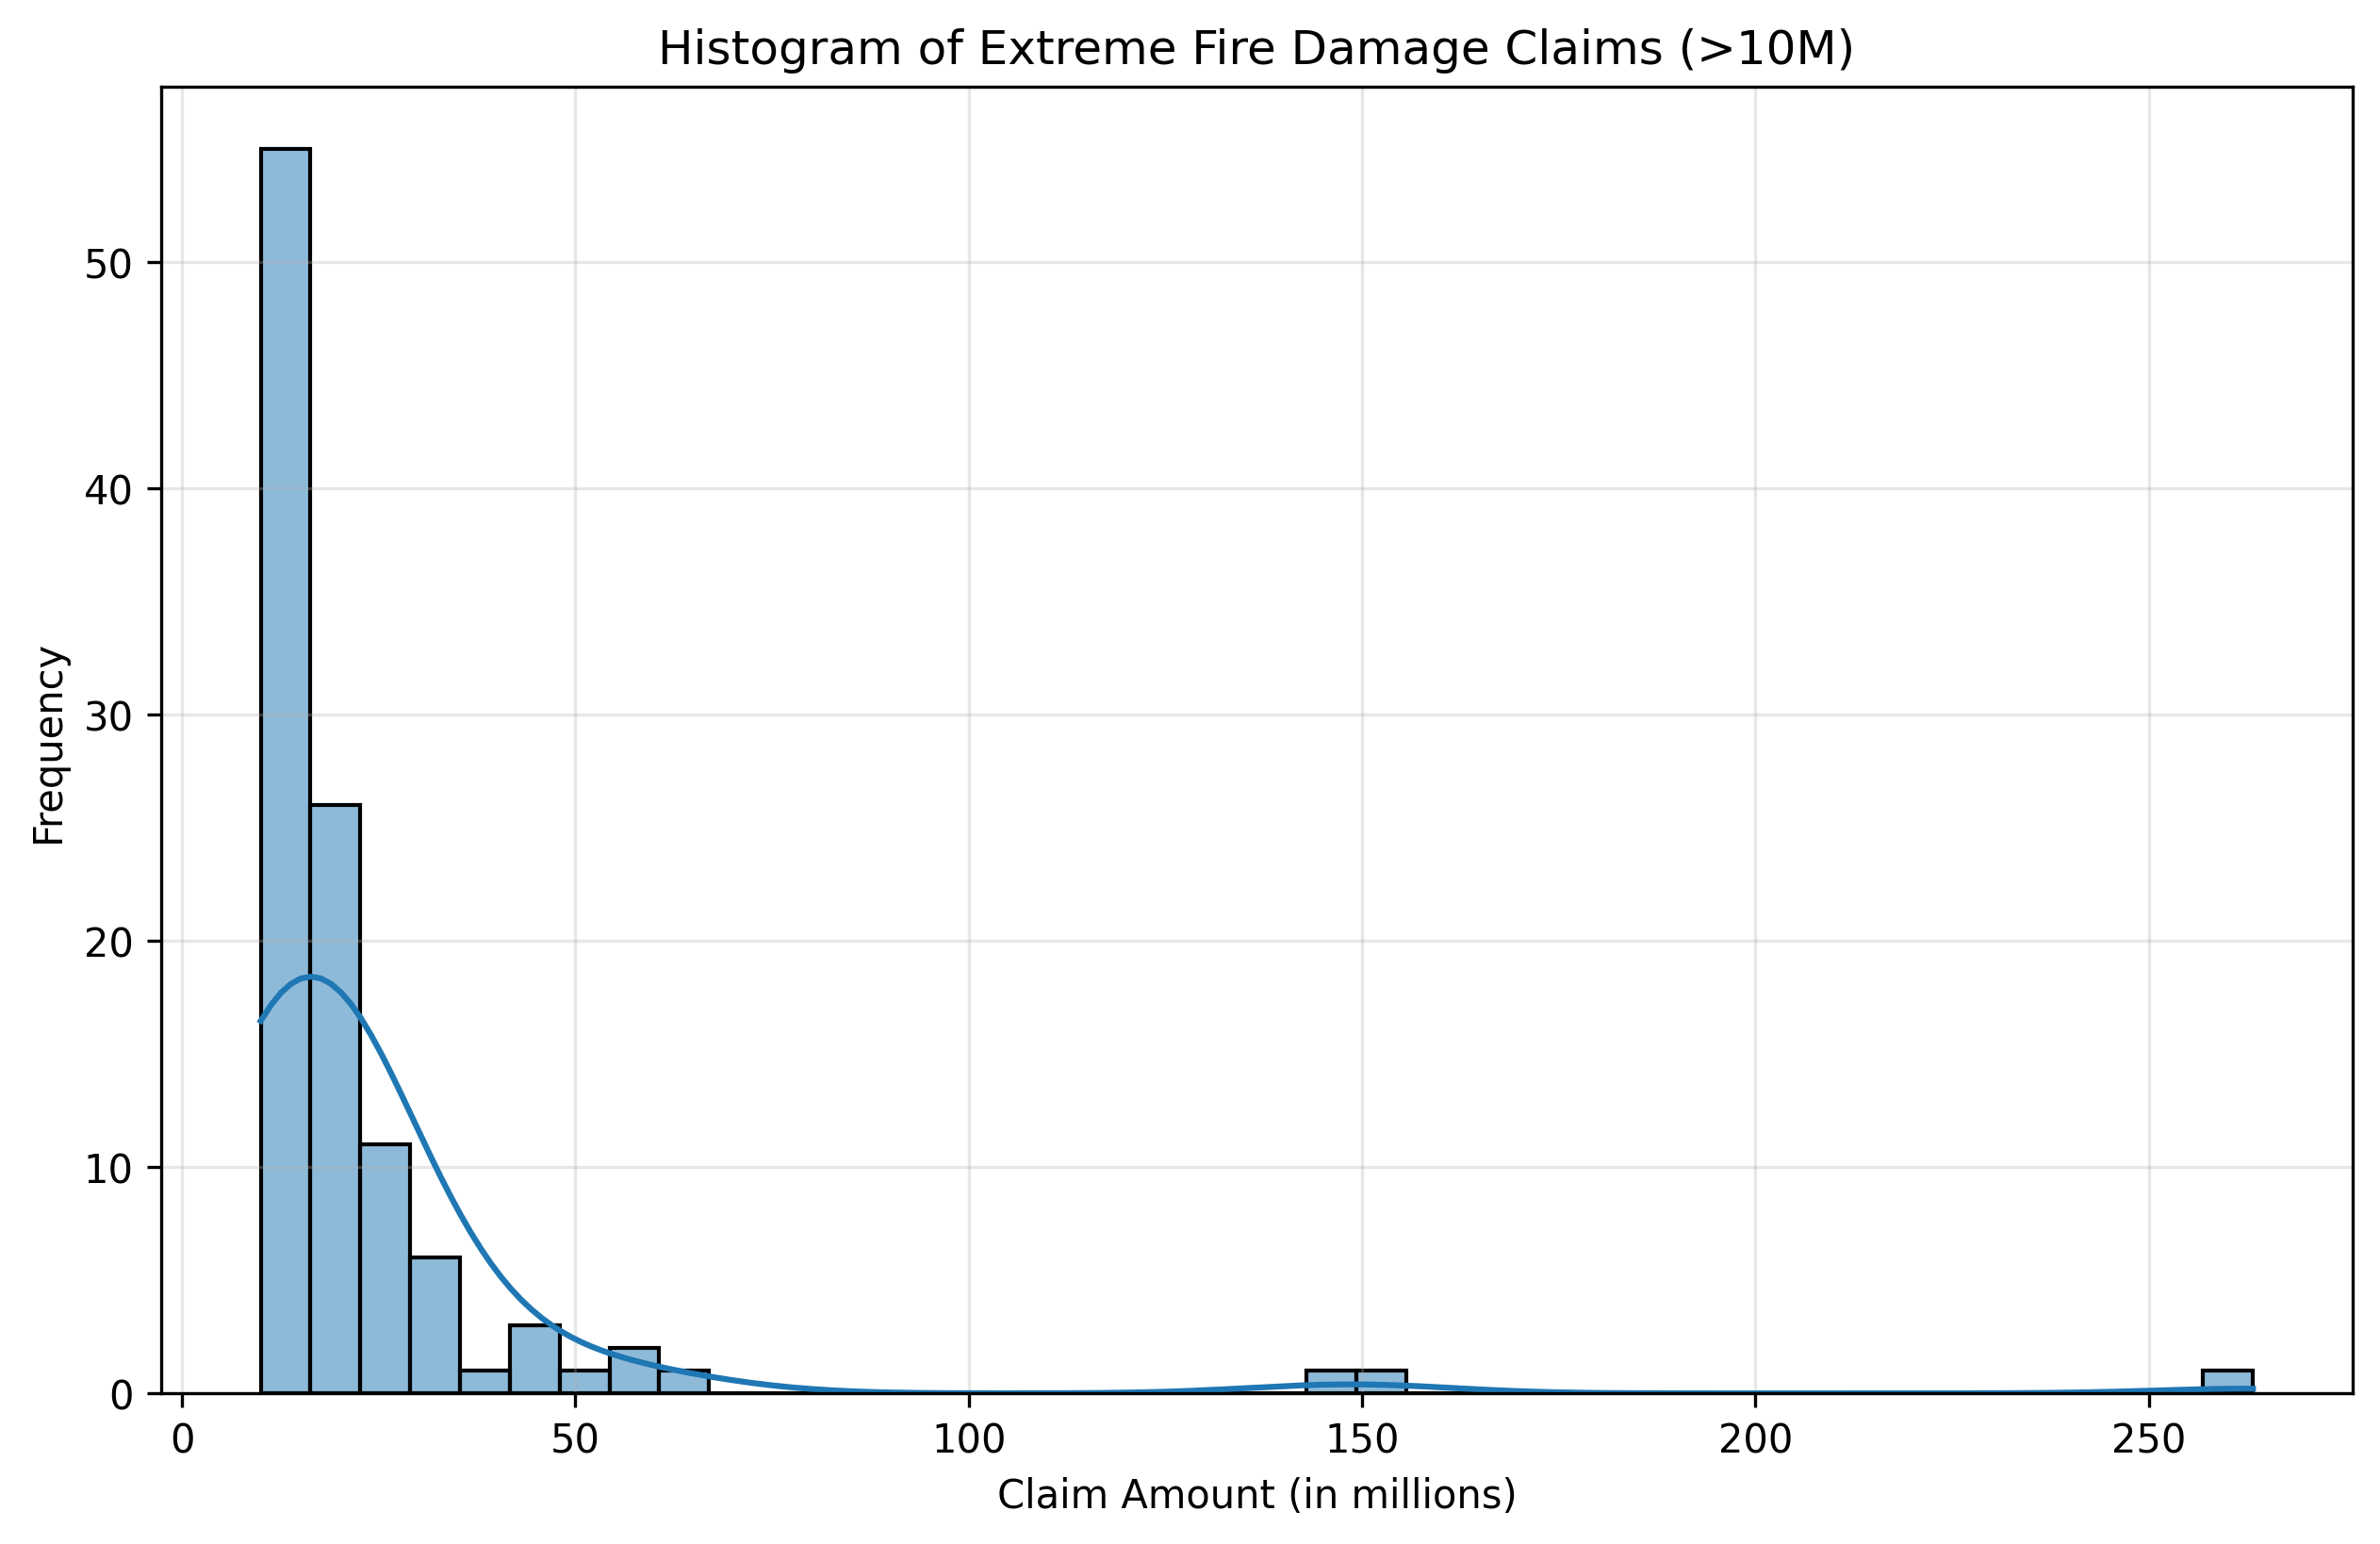
\includegraphics[width=\linewidth]{Figures/histogram_extreme.png}
        \caption{Extreme Fire Damage Claims ($>10$M)}
        \label{fig:histo-extreme}
    \end{minipage}
\end{figure}

The histograms in Figure~\ref{fig:histo-normal} and Figure~\ref{fig:histo-extreme} illustrate the distribution of claim amounts, separated into non-extreme and extreme values. Claims below 10 million DKK make up the majority of cases (95\%), while the extreme claims, though rare, contribute significantly to overall losses.

To better understand claim patterns over time, Figure~\ref{fig:historical-year} provides a yearly breakdown of total claims.

\begin{figure}[h]
    \centering
    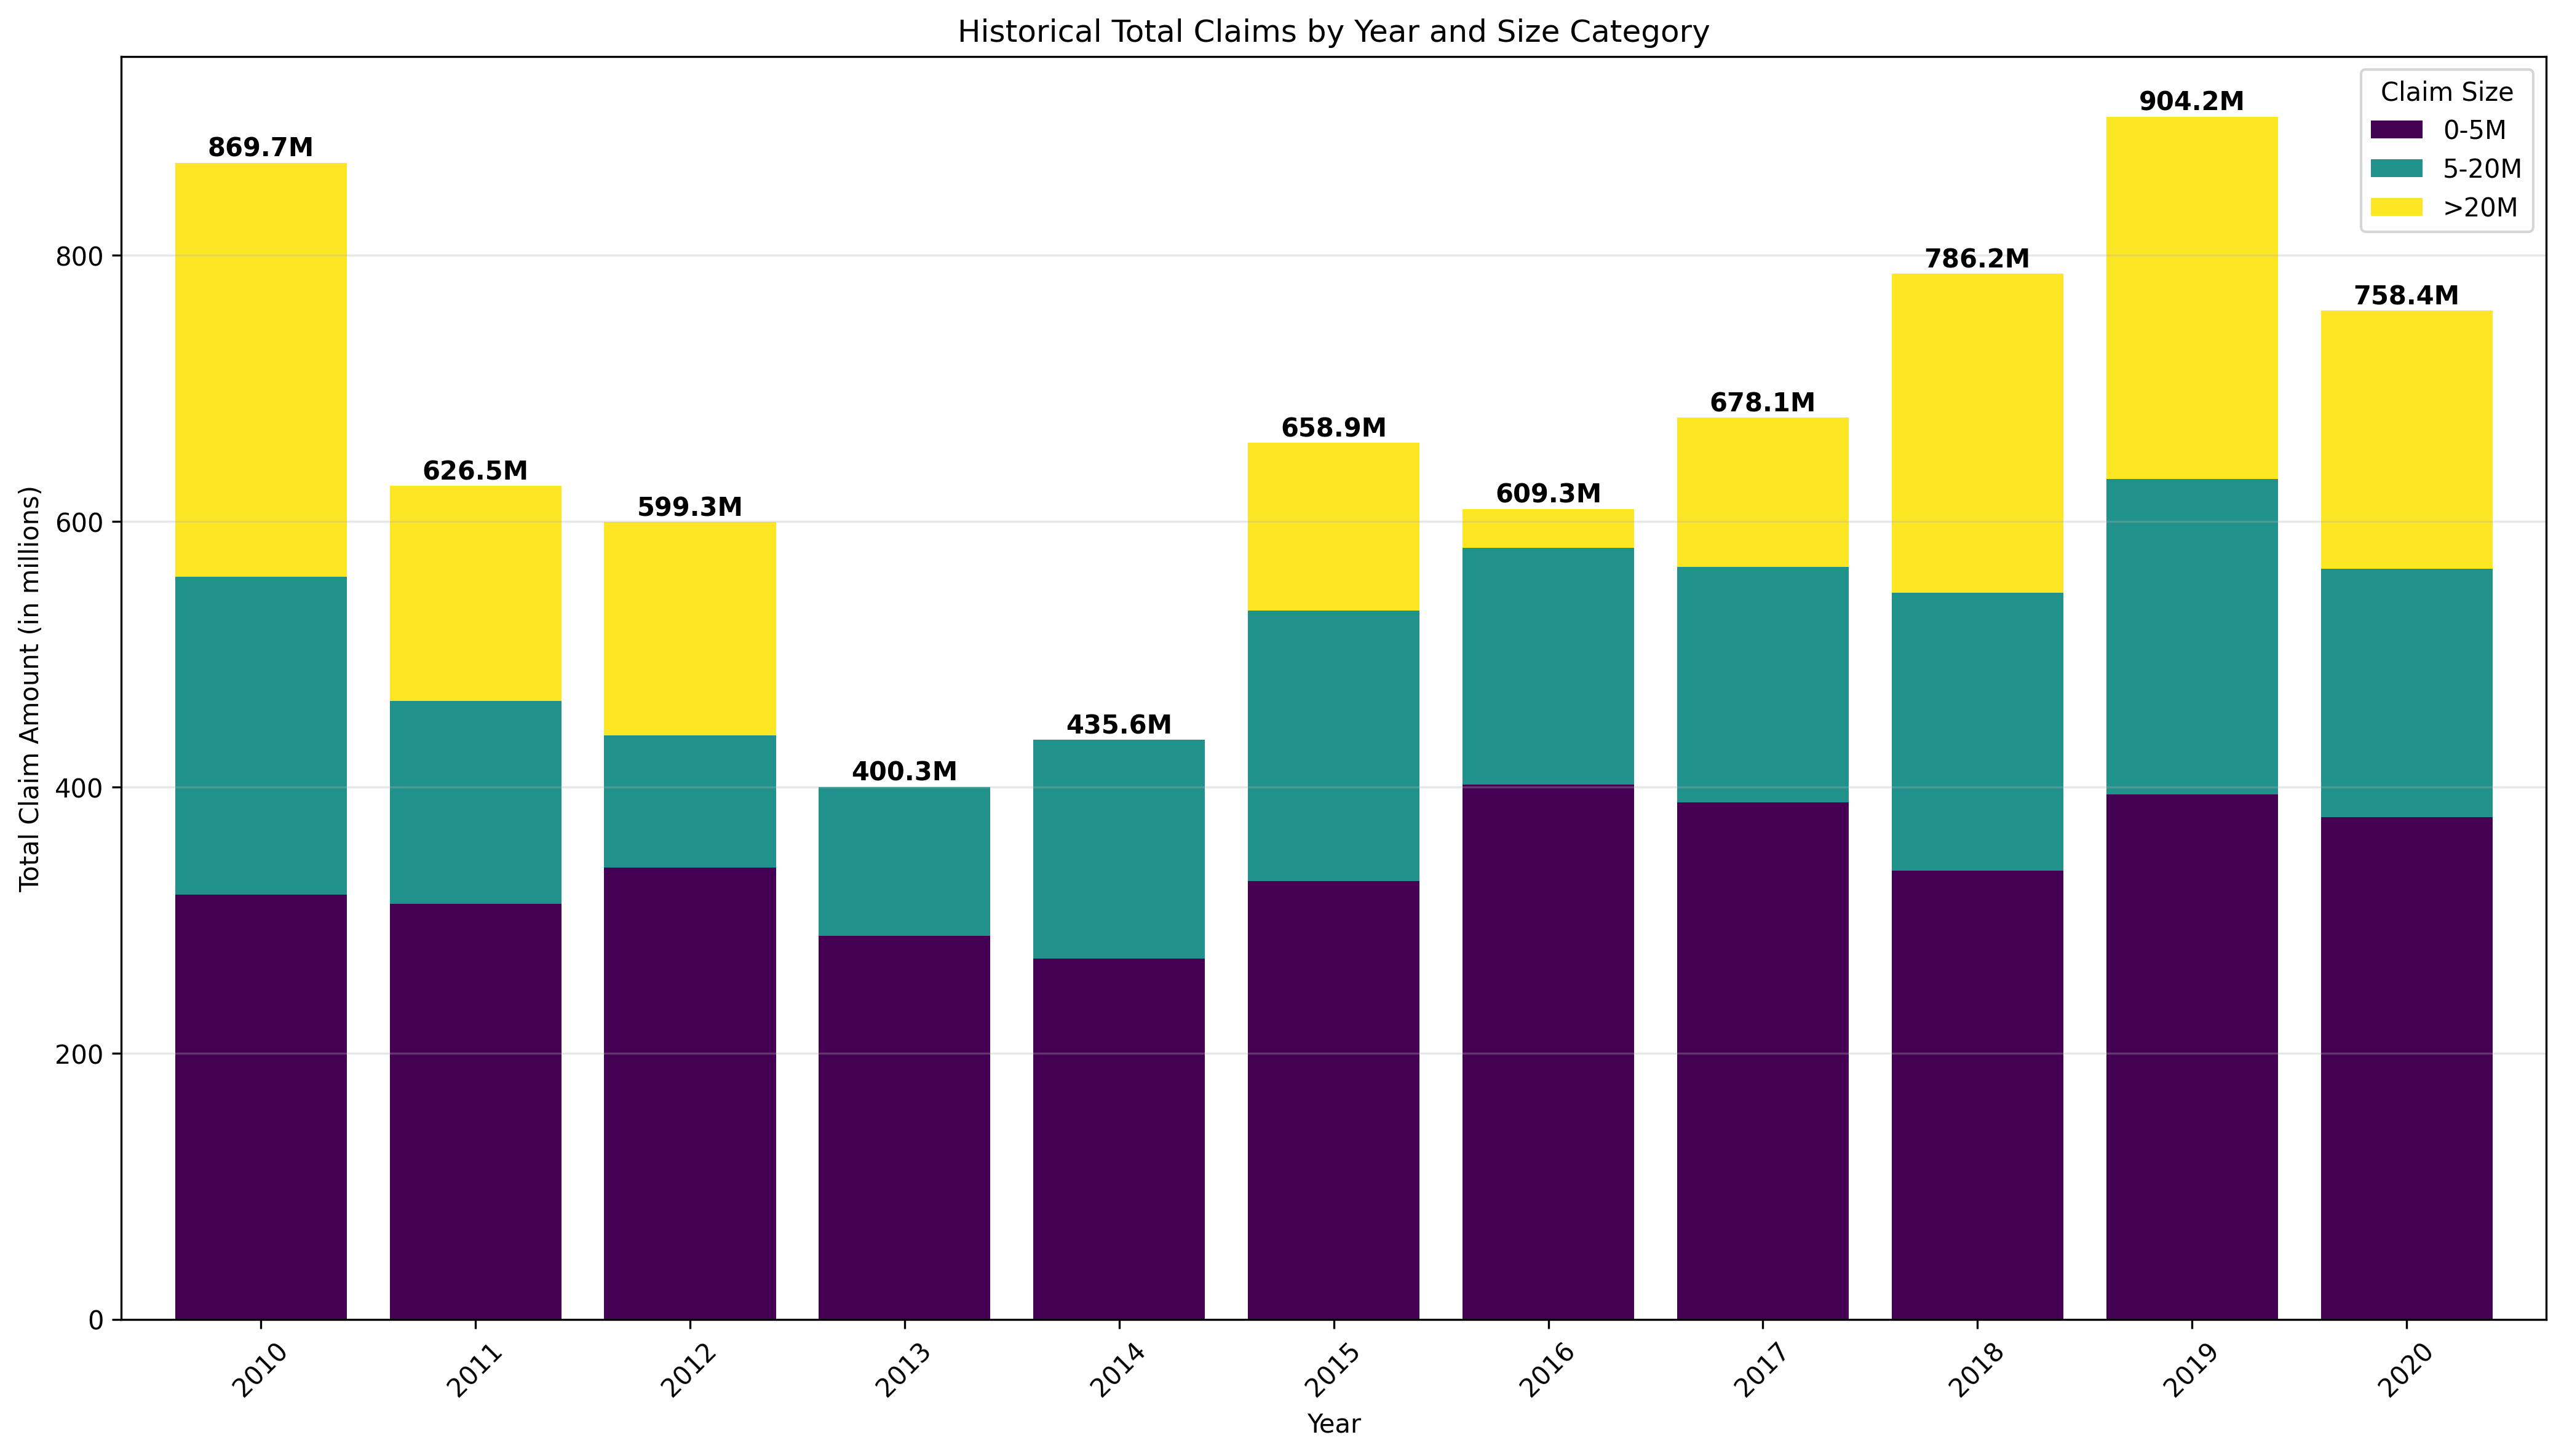
\includegraphics[width=0.6\textwidth]{Figures/historical_year_comparison.png}
    \caption{Total Fire Damage Claims by Year (2010-2020)}
    \label{fig:historical-year}
\end{figure}

The historical data reveals that claim amounts fluctuate over time, with some years experiencing significantly fewer large claims (e.g., 2013 and 2014). Understanding such variations is essential for risk assessment.

\subsubsection{Expected Loss Calculation}
Given that claim frequency follows a Poisson distribution with an expected number of claims per year:
\[
\lambda = \frac{900}{10^6} \times 630\,000 = 567
\]
The total expected loss each year without reinsurance is computed as:
\[
E[S] = \lambda \cdot E[X] = 567 \times 3.39 = 1\,919.67 \text{ million DKK}
\]
where the expected loss per claim, $E[X]$, is calculated empirically from the dataset.

The variance of total losses per year is then computed as:
\[
\operatorname{Var}(S) = \lambda E[X^2] = 567 \times 83.90 = 47\,569.83 \text{ million DKK}^2
\]
where the expected loss of individual claims squared, $E[X^2]$, is also derived empirically.

% This shouldn'y be mentioned here
% Applying Excess-of-Loss (XL) reinsurance, the expected loss and variance decrease significantly, as shown in Table \ref{tab:risk-metrics}.

\subsection{Distribution Approximation}
The accurate modeling of claim severity is crucial for risk assessment. Rather than using a single theoretical distribution for all claims, we explored multiple modeling approaches and evaluated their performance using a holdout set.

\subsubsection{Modeling Approaches}
We split the data into 50\% training and 50\% test sets to evaluate different modeling approaches:

\begin{enumerate}
    \item \textbf{Pure Empirical:} Using the empirical distribution from the training set with no parametric assumptions.
    \item \textbf{Hybrid Model:} Empirical distribution for common claims, theoretical distribution for extreme claims.
    \item \textbf{Two-Part Theoretical:} Different theoretical distributions for non-extreme and extreme claims.
    \item \textbf{Single Theoretical:} One parametric distribution for all claims.
\end{enumerate}

For the hybrid model, we tested different percentile thresholds to determine the optimal split point between empirical and theoretical components. Performance was evaluated using multiple metrics including Wasserstein distance, KL divergence, and relative errors in key statistics (mean, standard deviation, and high quantiles).

\subsubsection{Optimal Model Selection}
Cross-validation consistently showed that the hybrid approach outperformed other methods, with the configuration:
\begin{itemize}
    \item 97\% of claims (below 14.29M DKK) modeled using the empirical distribution
    \item 3\% of claims (above 14.29M DKK) modeled using a fitted log-normal distribution
\end{itemize}

This 97/3 hybrid approach provides the best of both worlds: data-driven modeling for common claims where we have abundant observations, and theoretical extrapolation for extreme events where data is sparse.

\begin{figure}[h]
    \centering
    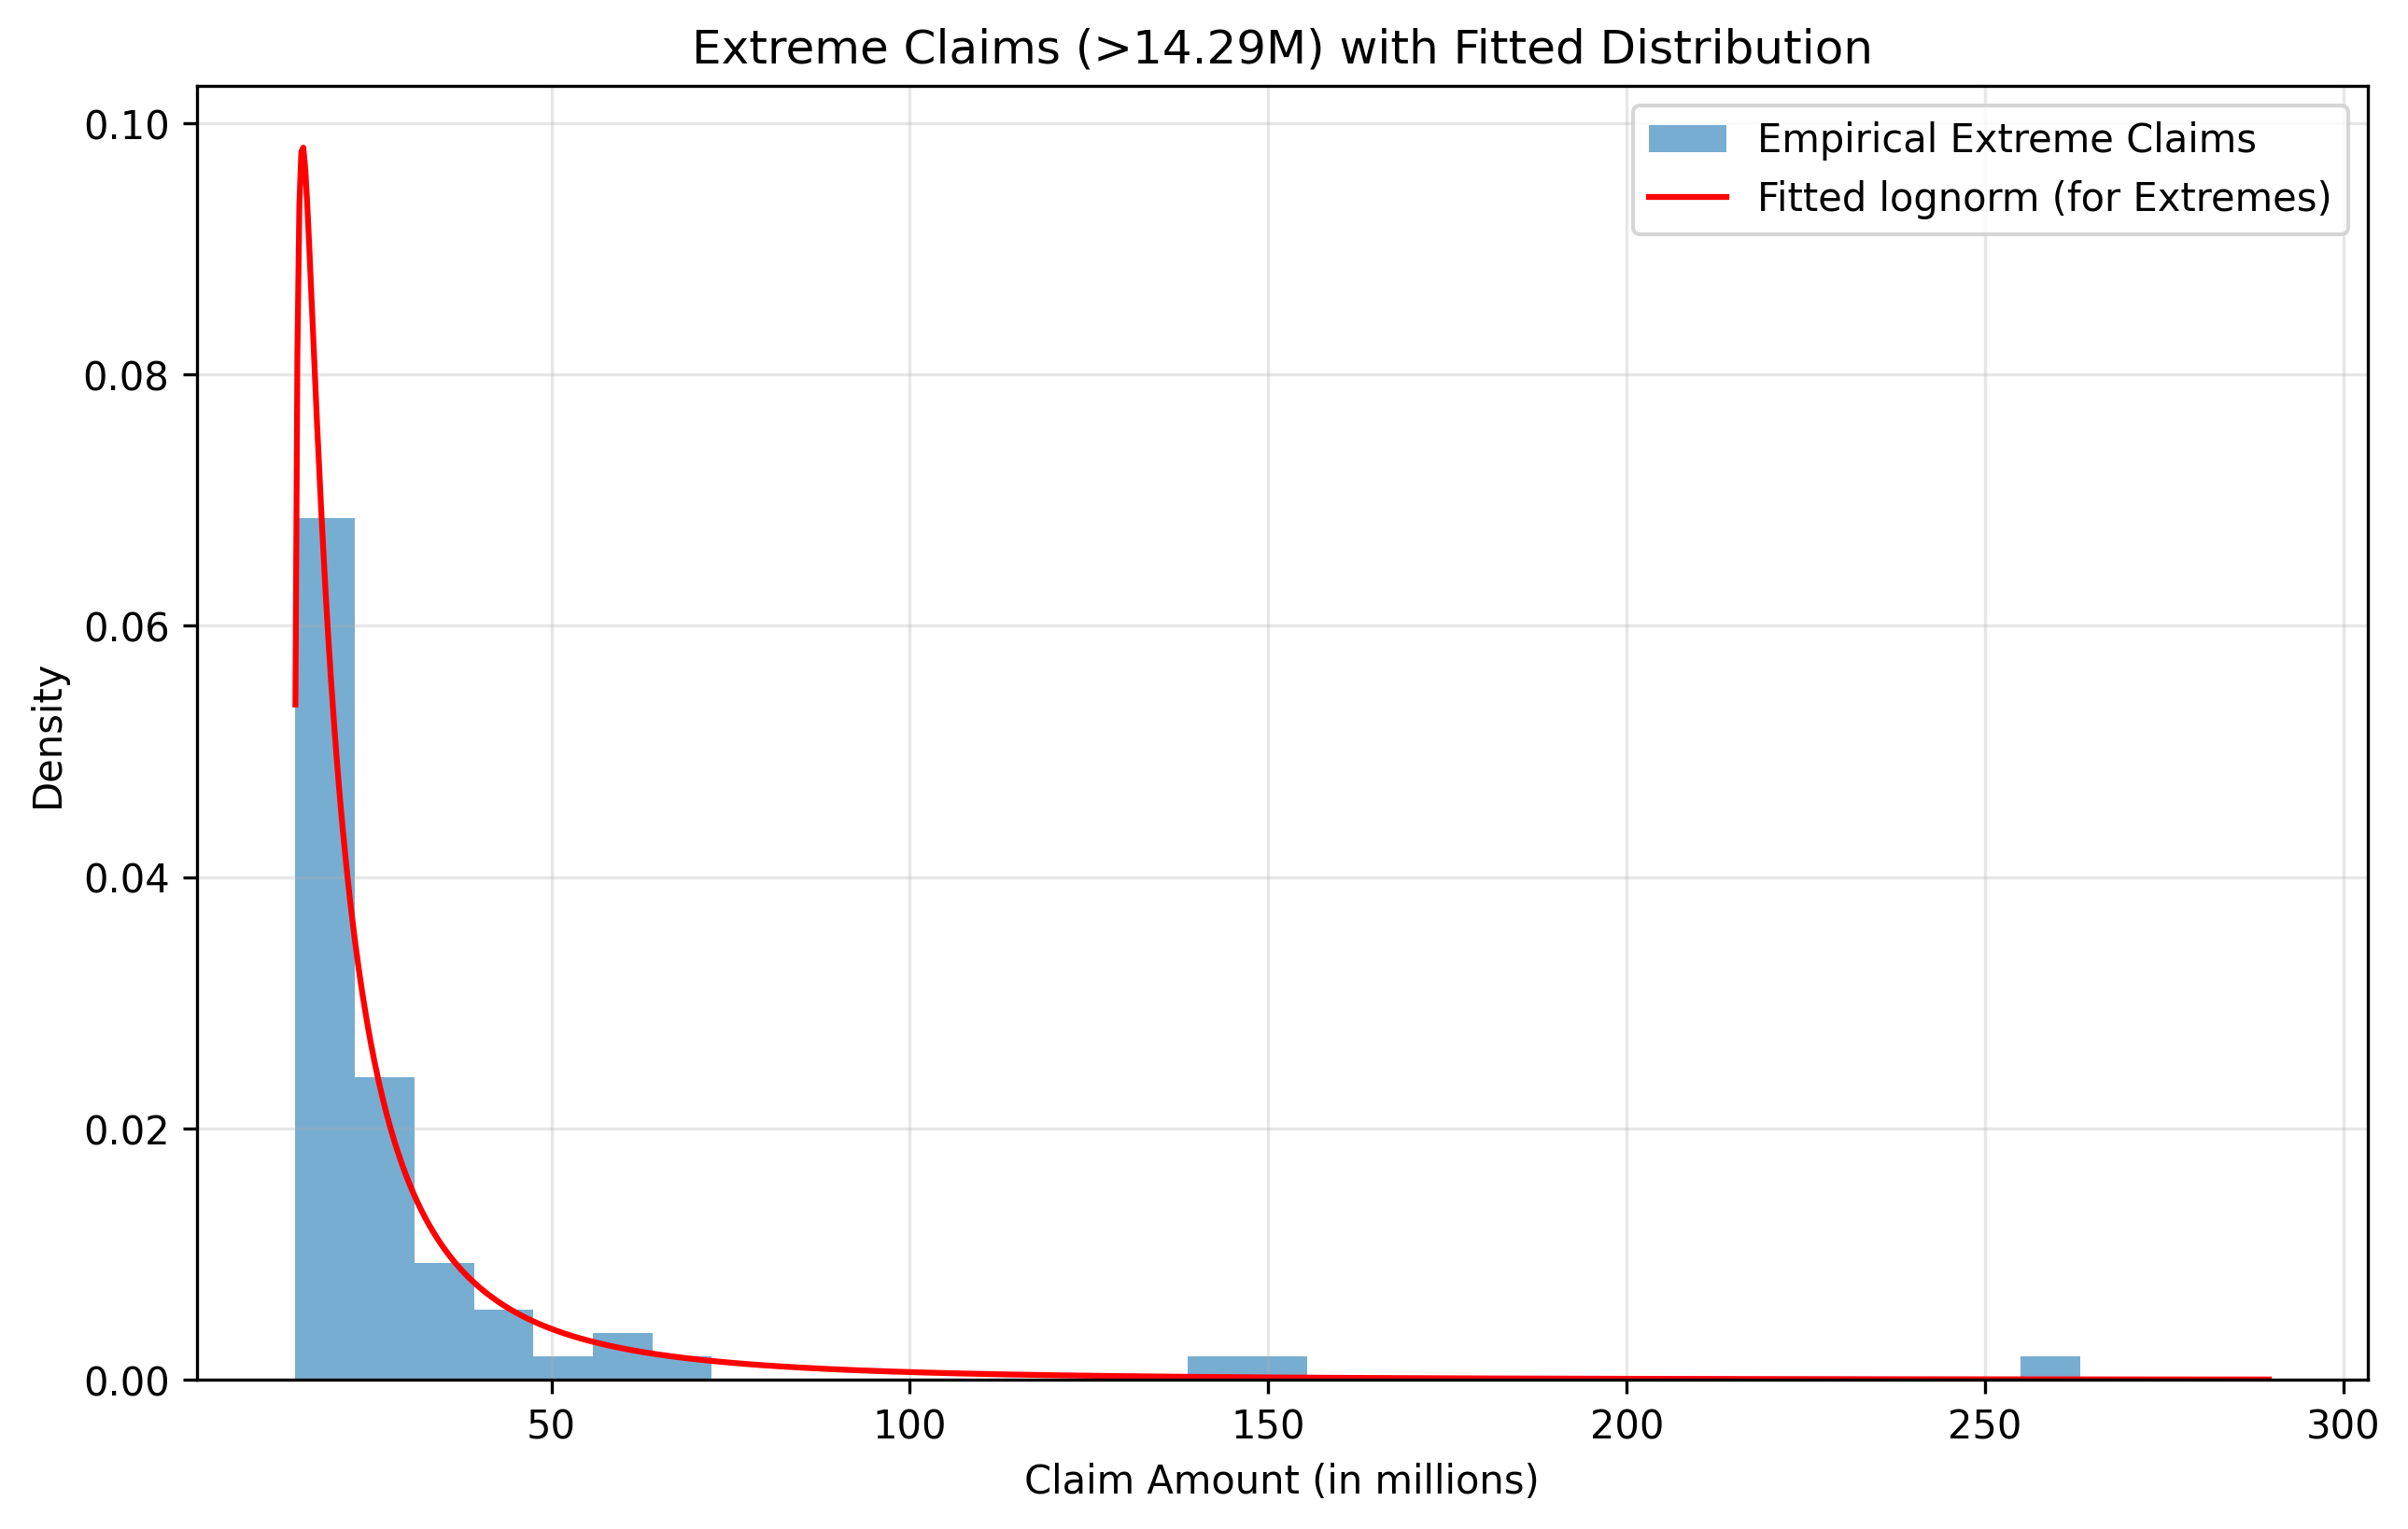
\includegraphics[width=0.5\textwidth]{Figures/extreme_claims_fit_97.png}
    \caption{Extreme claims (>14.29M) fitted with a log-normal distribution.}
    \label{fig:extreme-fit}
\end{figure}

%%

Figure~\ref{fig:extreme-fit} shows how the log-normal distribution fits the extreme claims. While different theoretical distributions (Pareto, generalized Pareto) were competitive for modeling extreme values, the log-normal consistently performed well across different splits of the data.

The resulting total loss distribution from this hybrid approach is shown in Figure~\ref{fig:total-claims-dist}.

%%

\subsection{Reinsurance Modeling and Financial Impact}
Reinsurance reduces risk exposure by capping individual claim payments. The reinsured loss per claim, $X_{XL}$, follows:

\[
X_{XL} =
\begin{cases}
0 & \text{if } X \leq M \\
X - M & \text{if } M < X \leq M + L \\
L & \text{if } X > M + L
\end{cases}
\]

Figure~\ref{fig:reinsurance-density} compares the total claim amounts retained by the insurer under different reinsurance scenarios.

\begin{figure}[h]
    \centering
    \begin{minipage}{0.48\textwidth}
        \centering        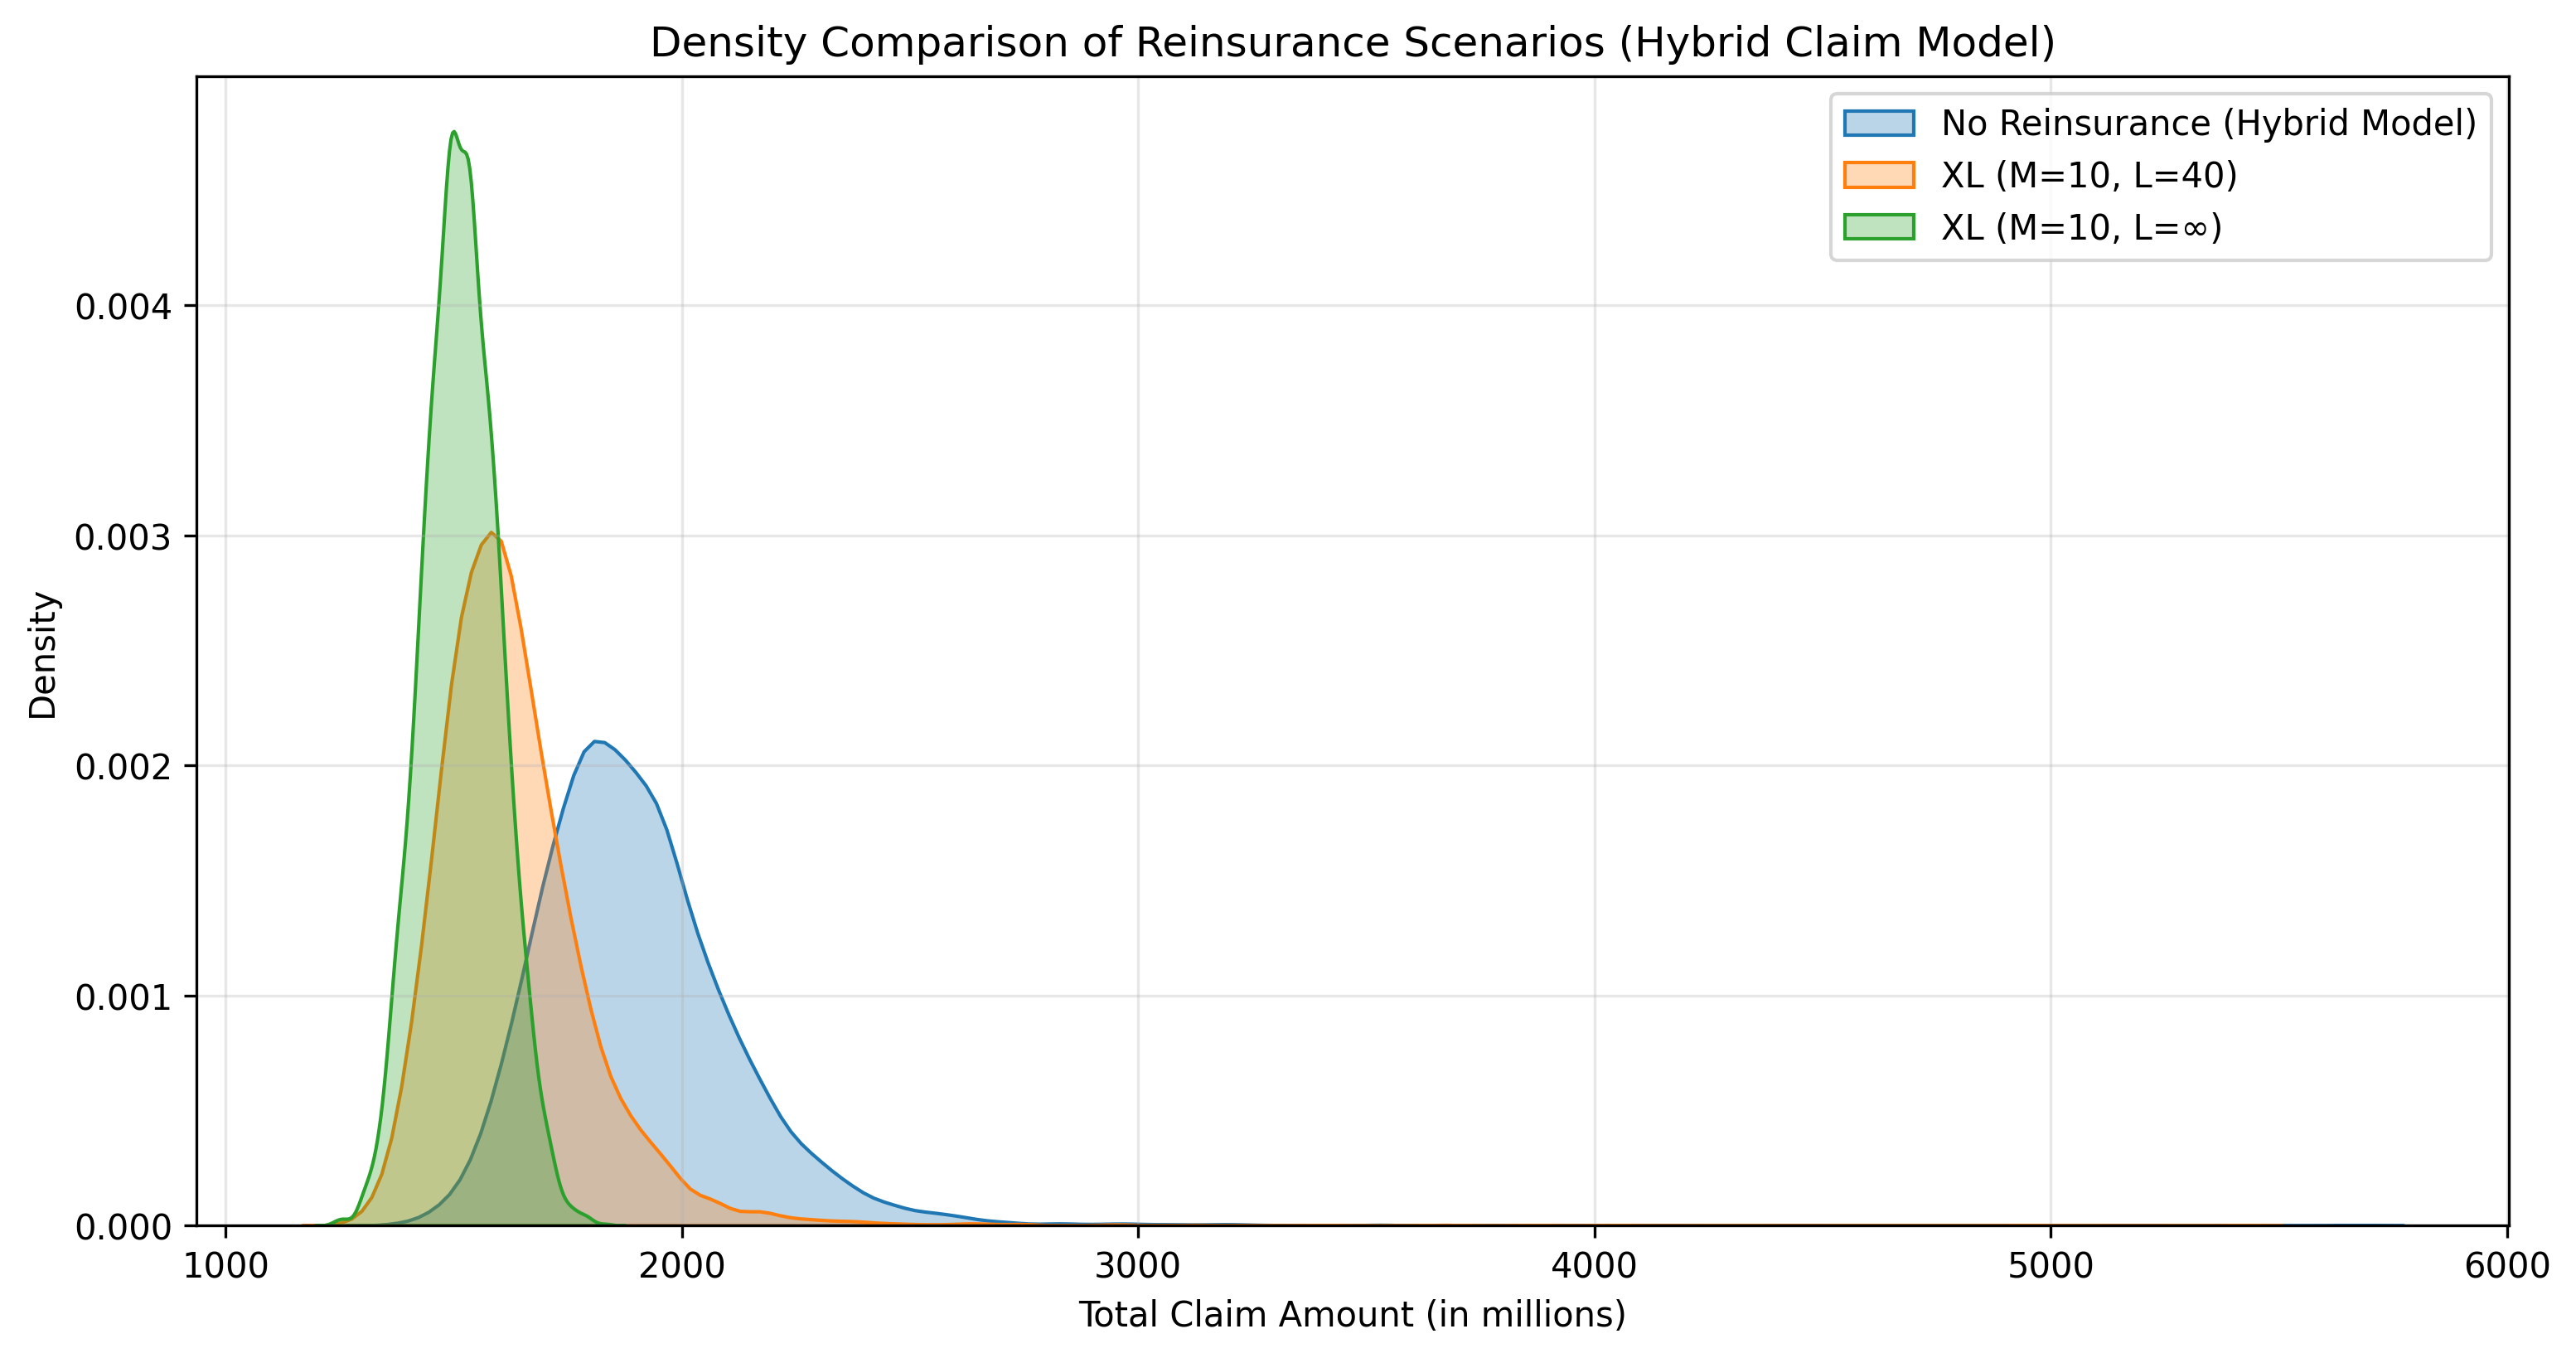
\includegraphics[width=\linewidth]{Figures/reinsurance_density.png}
        \caption{Density comparison of retained claims under different reinsurance scenarios.}
        \label{fig:reinsurance-density}
    \end{minipage}
    \hfill
    \begin{minipage}{0.48\textwidth}
        \centering
        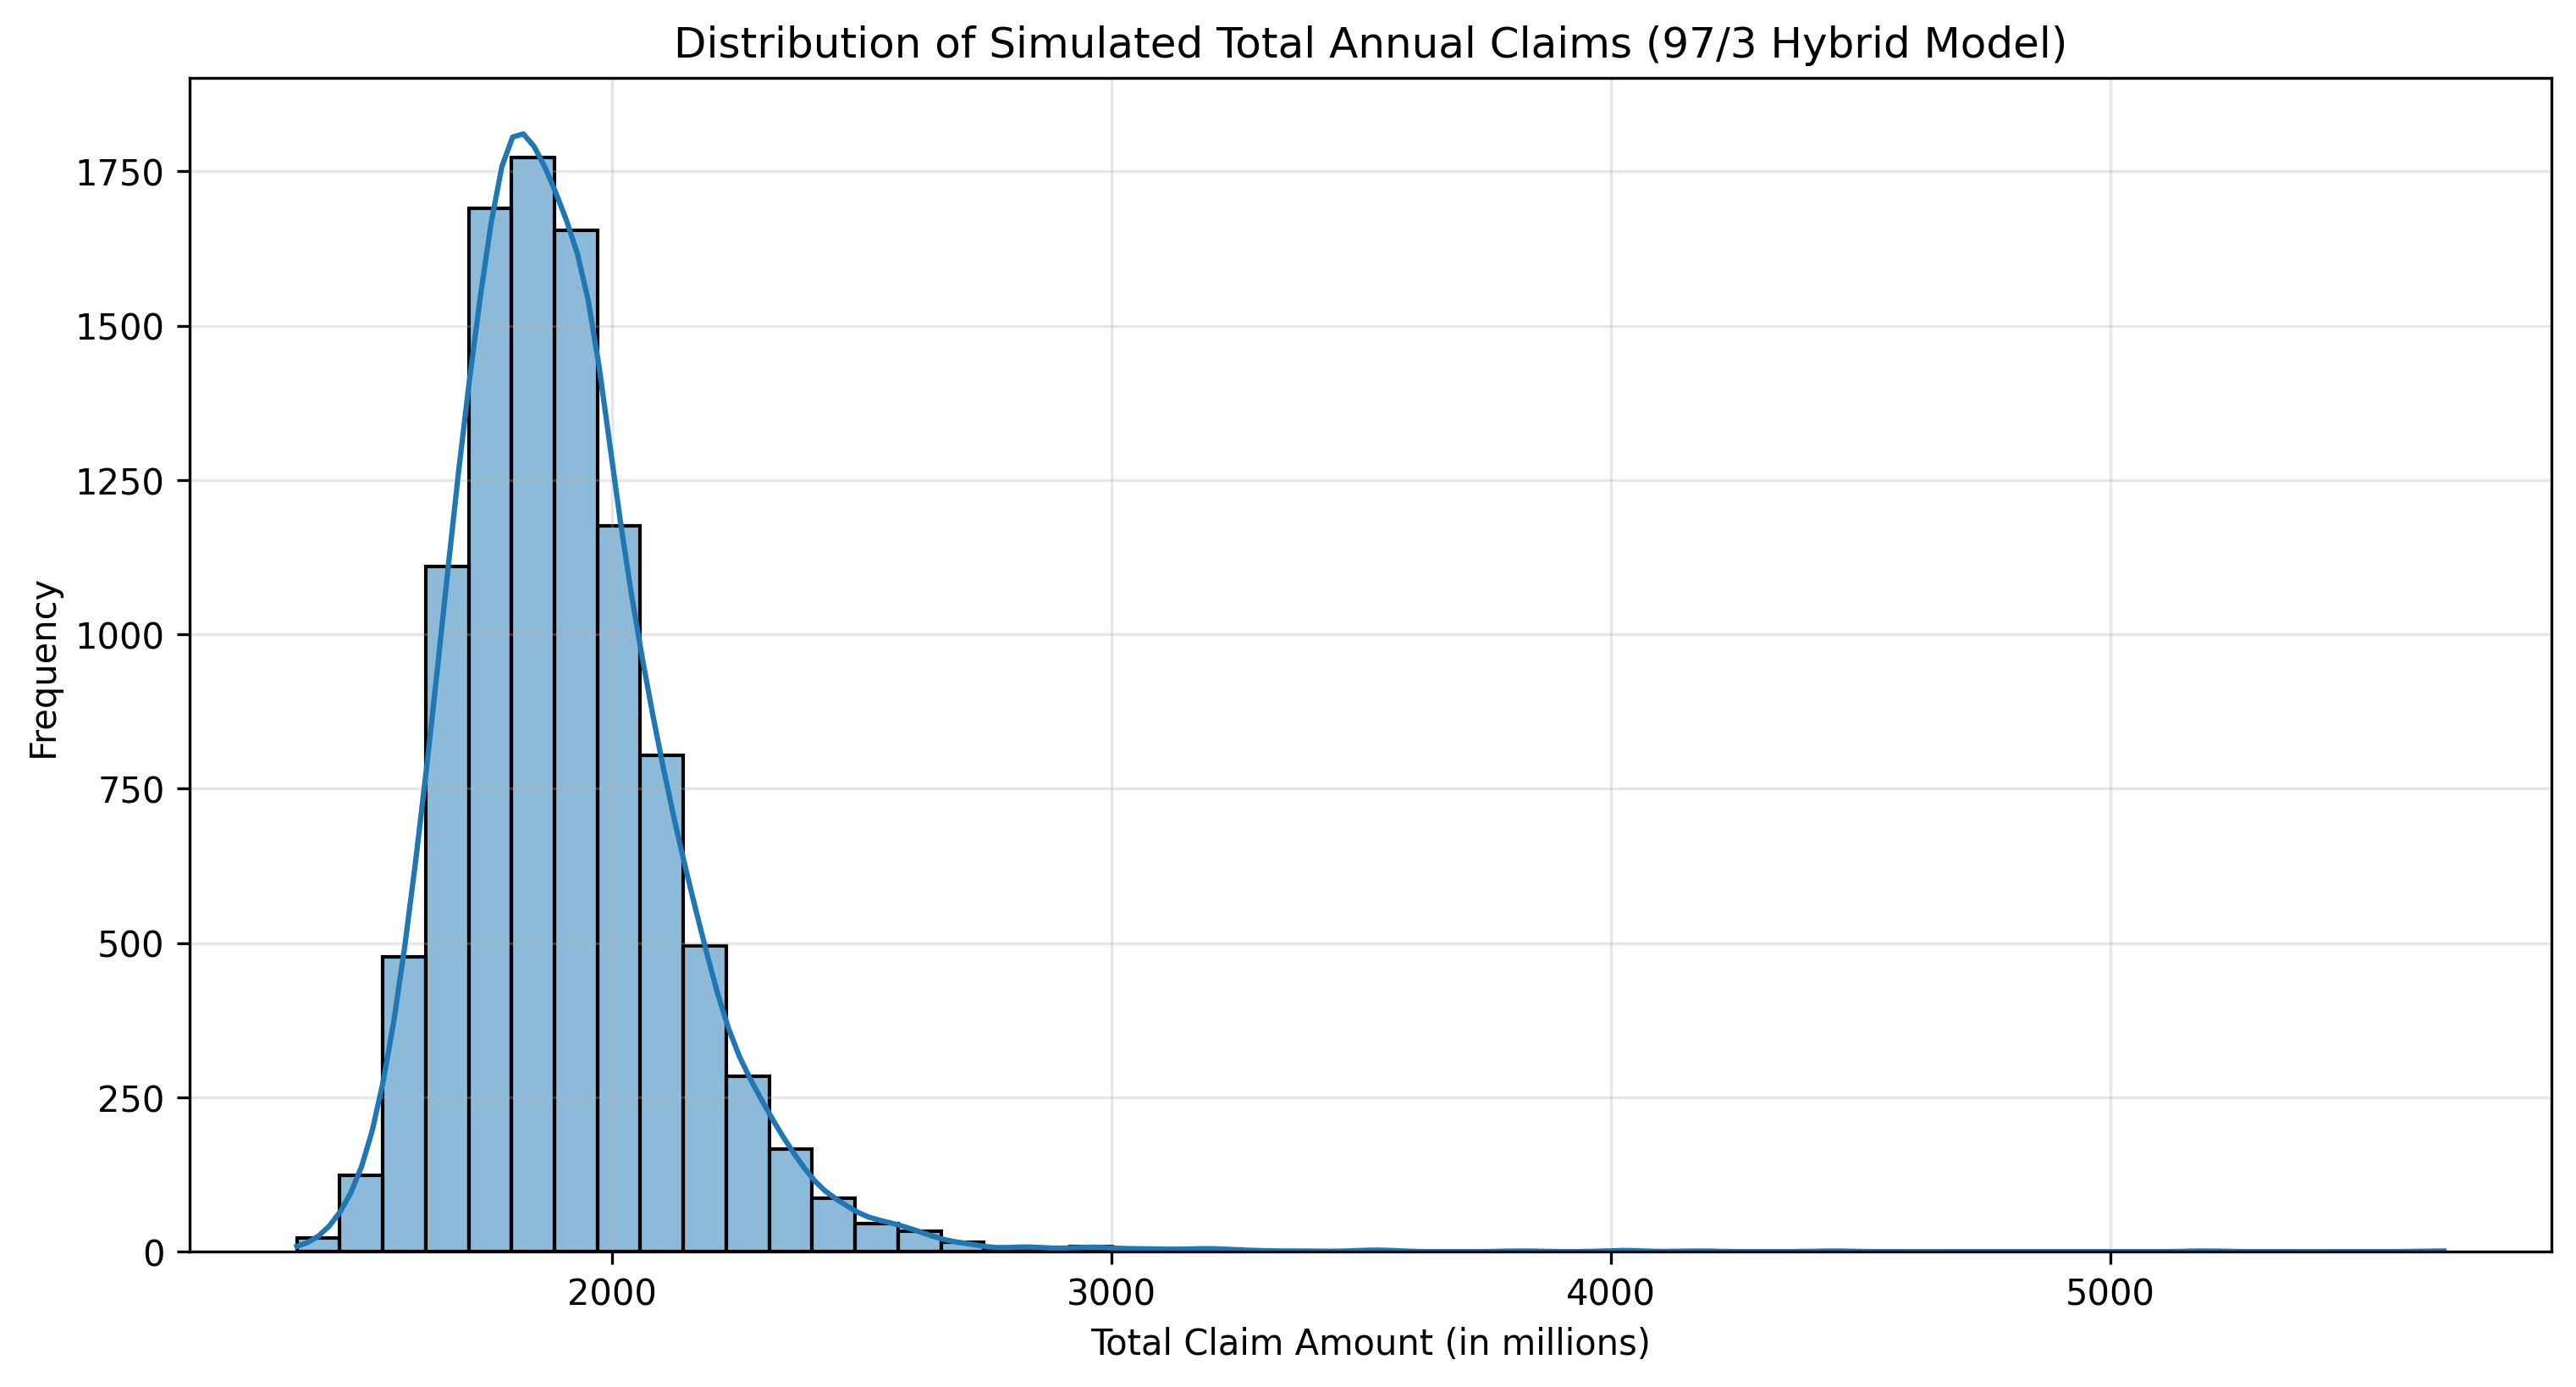
\includegraphics[width=\linewidth]{Figures/total_claims_distribution.png}
        \caption{Distribution of total annual claims generated using the 97/3 hybrid model.}
        \label{fig:total-claims-dist}
    \end{minipage}
\end{figure}

The density plot shows that Contract 1 ($M=10, L=40$) shifts the distribution to the left while maintaining a similar shape to the no-reinsurance scenario. Contract 2 ($M=10, L=\infty$), however, dramatically narrows the distribution, virtually eliminating the tail risk.

Using the hybrid claim simulation model, we derive risk metrics for each reinsurance scenario, shown in Table~\ref{tab:risk-metrics}



\begin{table}[h]
    \centering
    \begin{tabular}{lccc}
        \toprule
        \textbf{Metric} & \textbf{No Reinsurance} & \textbf{XL (M=10, L=40)} & \textbf{XL (M=10, L=$\infty$)} \\
        \midrule
        Expected Value & 1\,903.24 & 1\,632.83 & 1\,516.29 \\
        Standard Deviation & 223.69 & 179.64 & 83.02 \\
        Coefficient of Variation & 0.118 & 0.110 & 0.055 \\
        99\% VaR & 2\,552.92 & 2\,196.76 & 1\,713.60 \\
        Interquartile Range & 469.04 & 479.01 & 98.41 \\
        \bottomrule
    \end{tabular}
    \vspace{1em}
    \caption{Comparison of risk metrics under different reinsurance scenarios.}
    \label{tab:risk-metrics}
\end{table}

Table~\ref{tab:quantiles} provides a detailed comparison of key extreme quantiles across the reinsurance scenarios.

\begin{table}[h]
    \centering
    \begin{tabular}{lccc}
        \toprule
        \textbf{Quantile} & \textbf{No Reinsurance} & \textbf{XL (M=10, L=40)} & \textbf{XL (M=10, L=$\infty$)} \\
        \midrule
        50\% & 1877.40 & 1605.89 & 1515.57 \\
        90\% & 2168.56 & 1827.41 & 1624.83 \\
        95\% & 2280.37 & 1927.63 & 1655.93 \\
        99\% & 2556.76 & 2203.20 & 1716.43 \\
        99.5\% & 2708.07 & 2353.15 & 1738.61 \\
        99.9\% & 3213.13 & 2896.35 & 1787.87 \\
        \bottomrule
    \end{tabular}
    \vspace{1em}
    \caption{Quantiles of simulated total losses under different reinsurance structures (50,000 simulations).}
    \label{tab:quantiles}
\end{table}

\subsection{Revenue and Profit Analysis}

When selecting reinsurance contracts, insurers must balance risk reduction against profitability. We analyze the revenue implications of each reinsurance option, considering both premium income and costs.

Figure~\ref{fig:revenue-density} shows the distribution of insurance revenue (premium income minus claims and reinsurance costs) under each scenario. While the no-reinsurance option has the highest expected revenue, it also exhibits the widest spread, indicating greater volatility in financial outcomes.

To better understand the risk-return tradeoff, Figure~\ref{fig:revenue-quantile} provides a quantile plot of revenue.

\begin{figure}[h]
    \centering
    \begin{minipage}{0.48\textwidth}
        \centering
        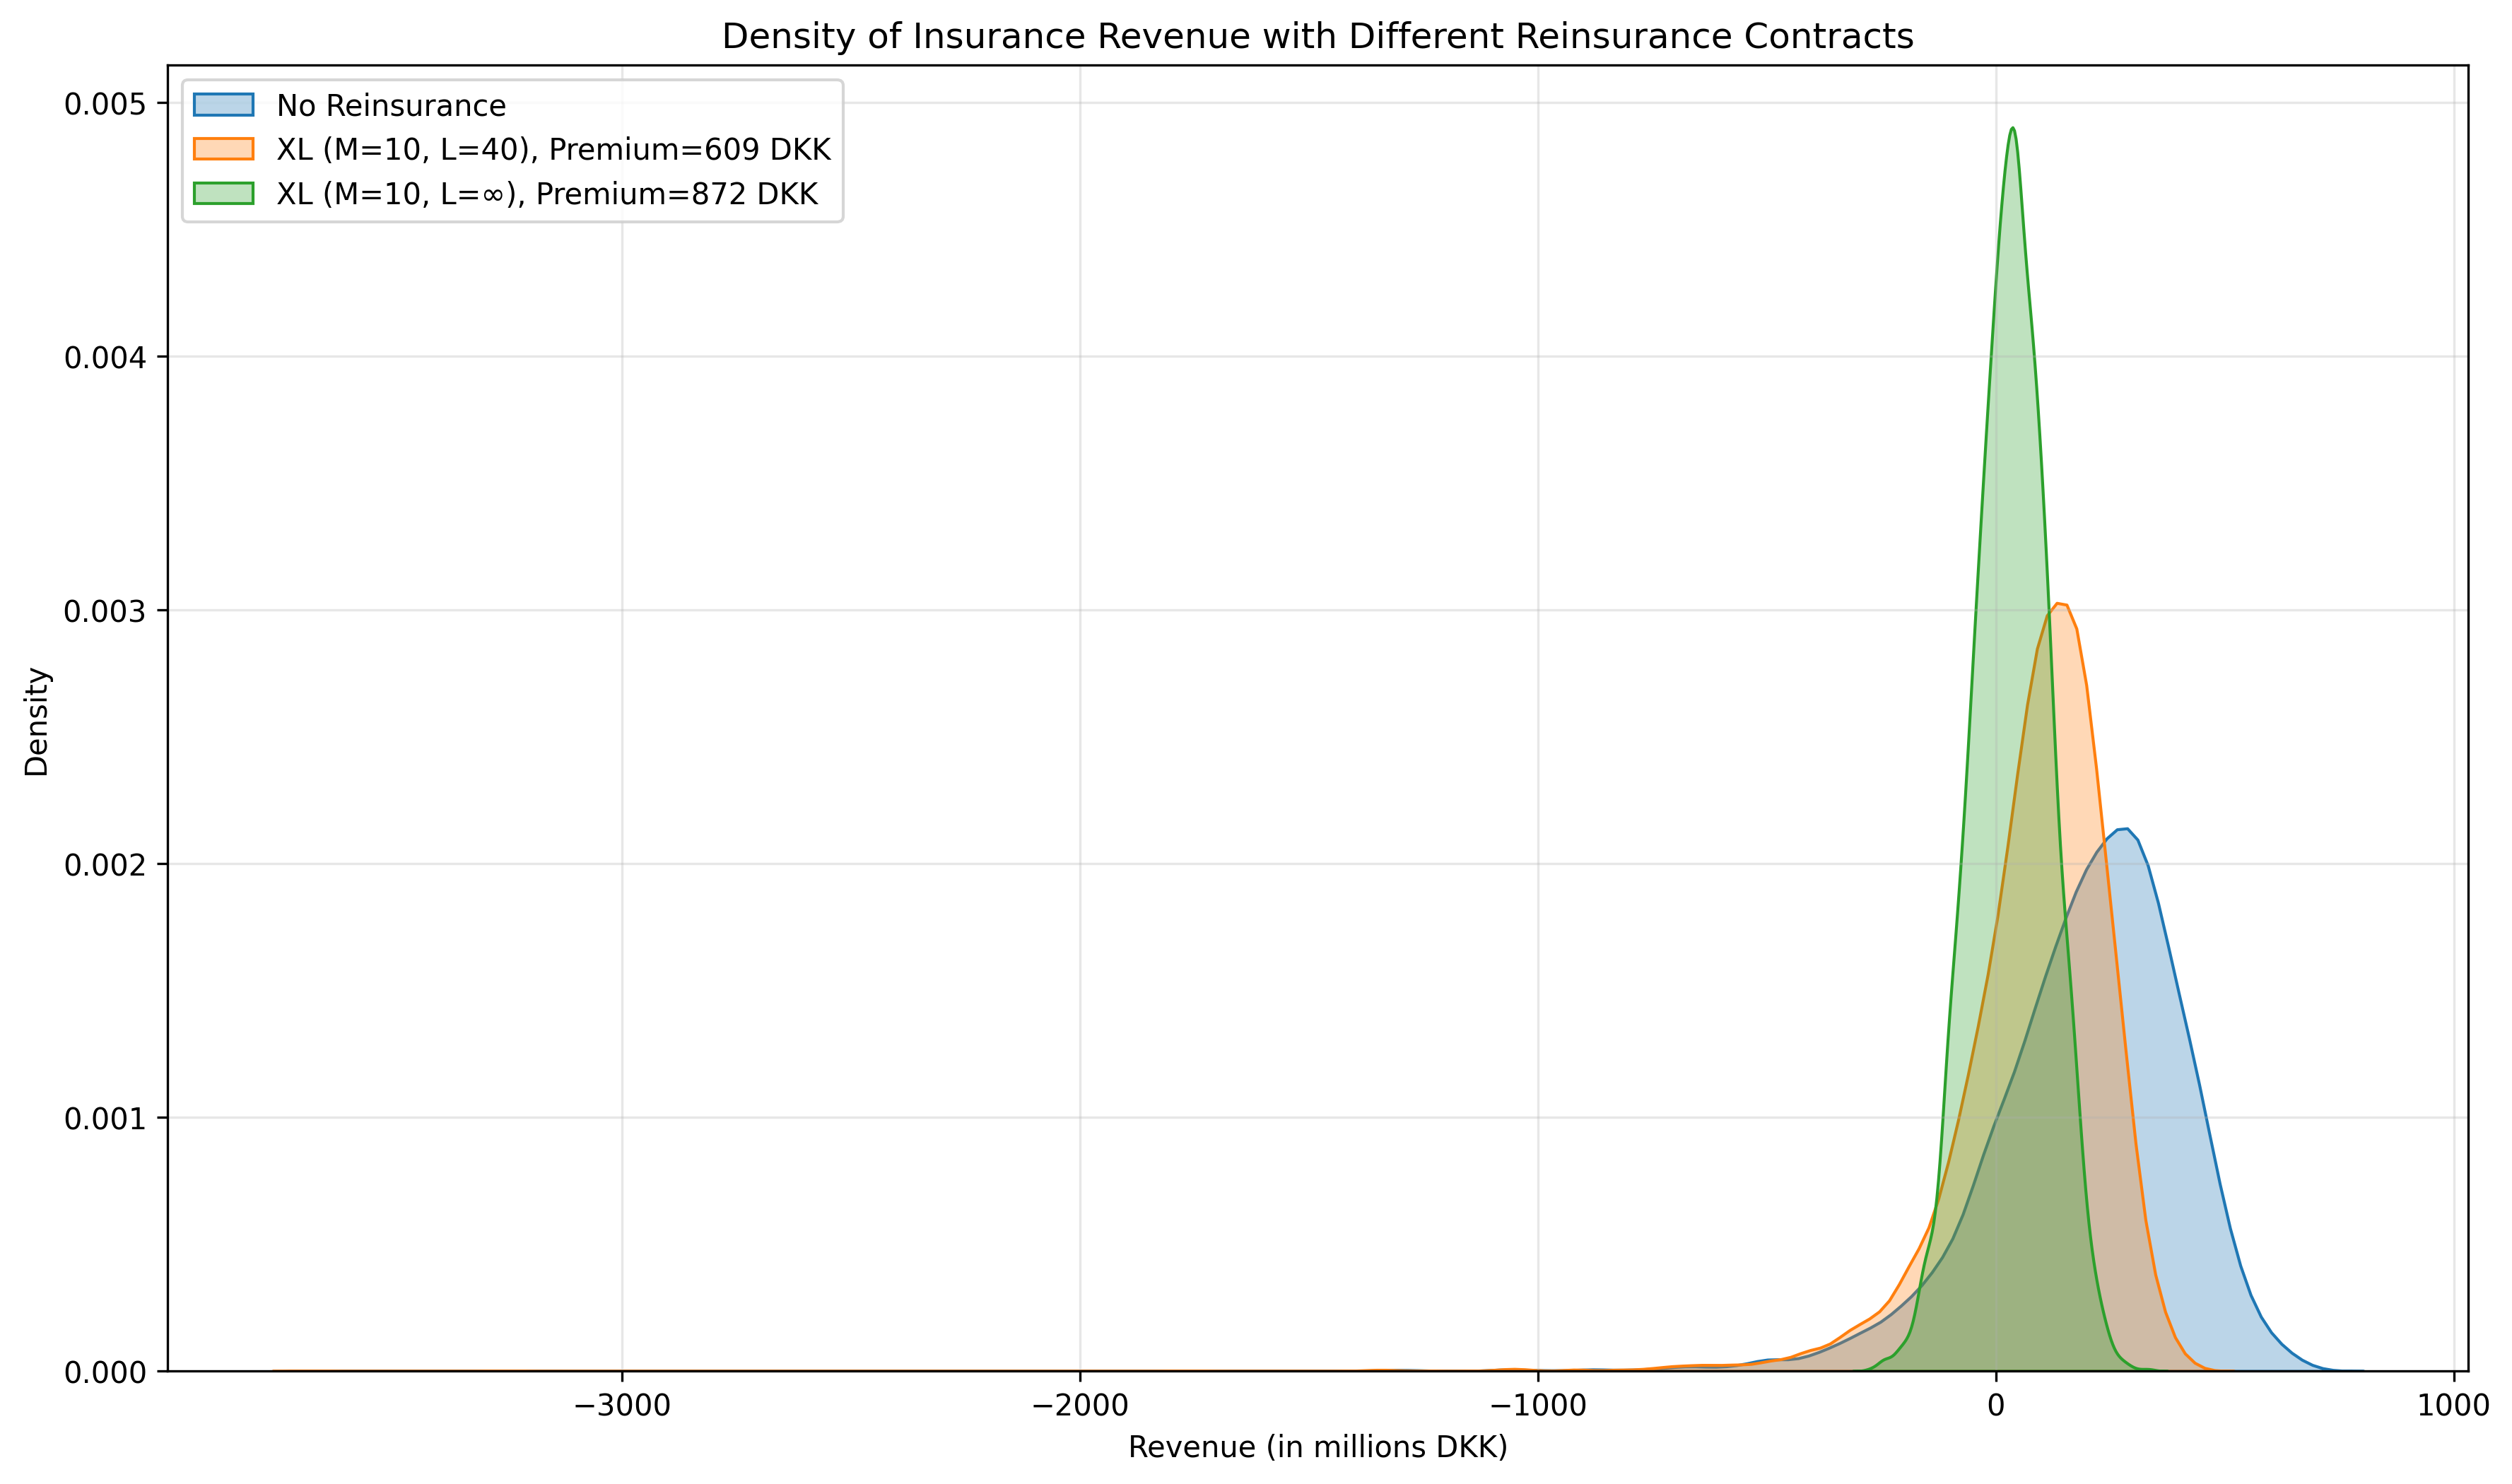
\includegraphics[width=\linewidth]{Figures/reinsurance_revenue_density.png}
        \caption{Density of insurance revenue with different reinsurance contracts.}
        \label{fig:revenue-density}
    \end{minipage}
    \hfill
    \begin{minipage}{0.48\textwidth}
        \centering
        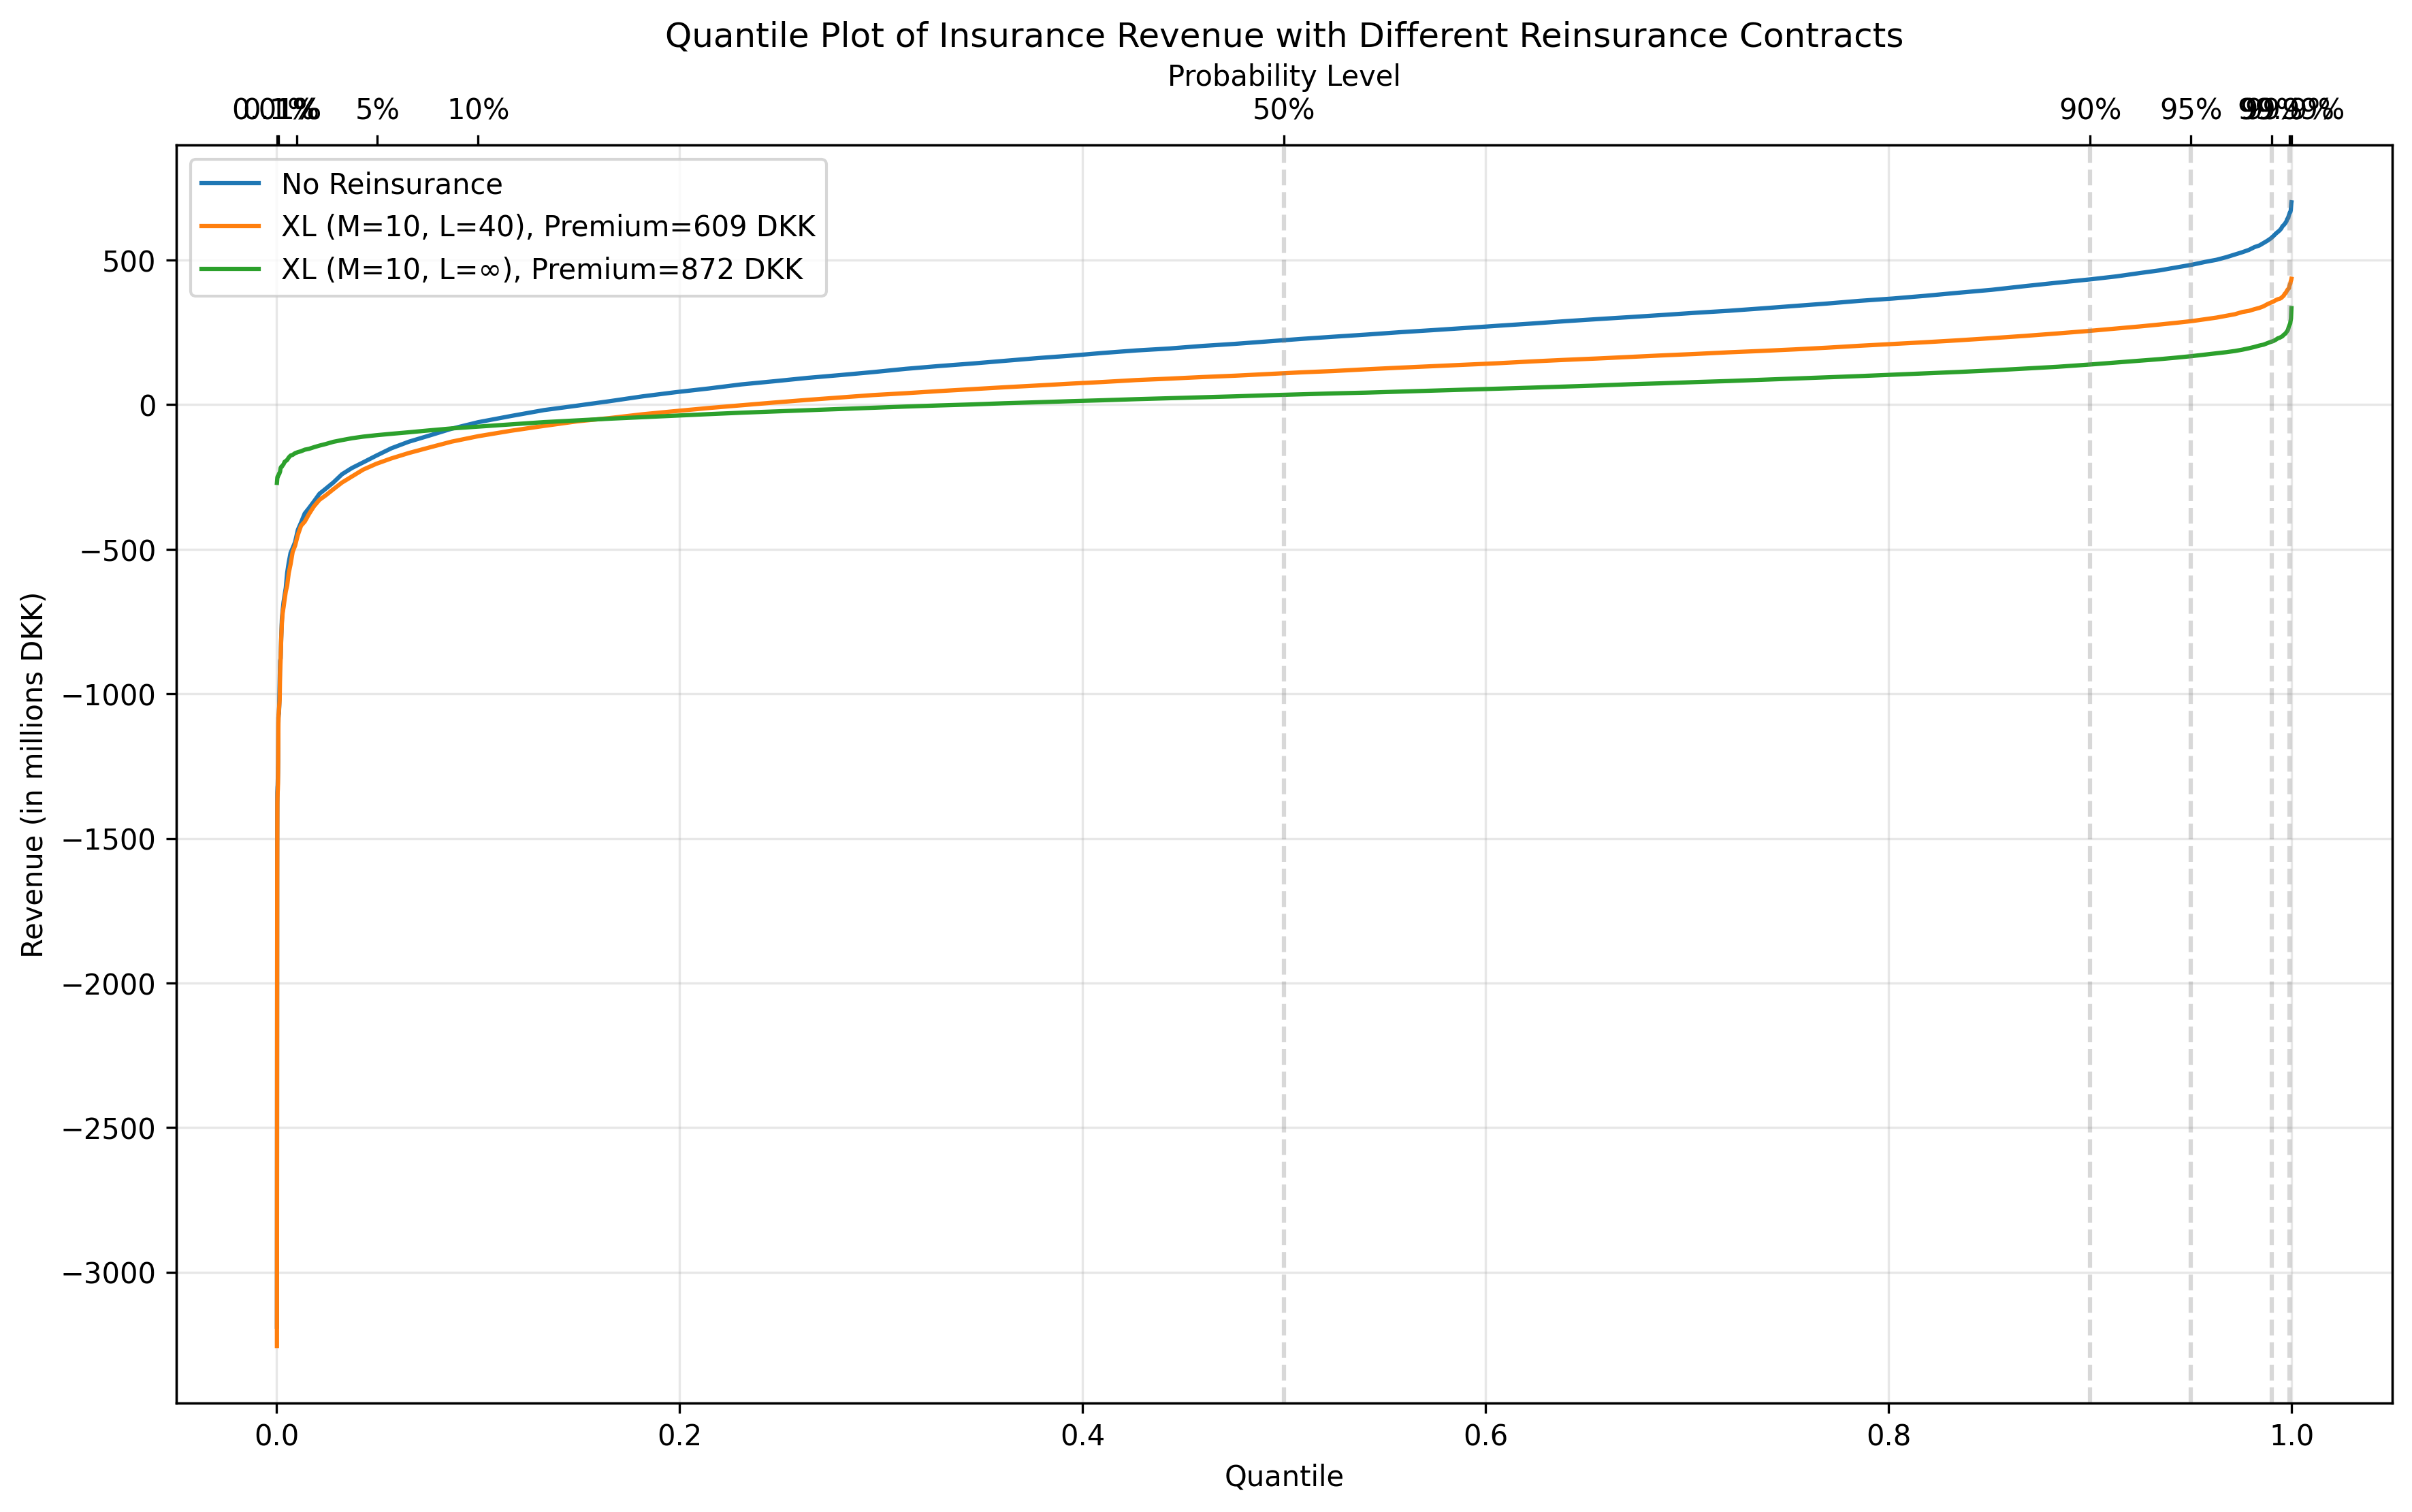
\includegraphics[width=\linewidth]{Figures/reinsurance_revenue_quantile.png}
        \caption{Quantile plot of insurance revenue with different reinsurance contracts.}
        \label{fig:revenue-quantile}
    \end{minipage}
\end{figure}

%

The quantile plot reveals that Contract 2 ($M=10, L=\infty$) offers superior protection against extreme losses, as shown by its much higher minimum revenue values. This comes at the cost of lower expected revenue.

\begin{table}[h]
    \centering
    \begin{tabular}{lccc}
        \toprule
        \textbf{Metric} & \textbf{No Reinsurance} & \textbf{XL (M=10, L=40)} & \textbf{XL (M=10, L=$\infty$)} \\
        \midrule
        Expected Revenue & 195.29 & 82.03 & 32.88 \\
        Standard Deviation & 223.69 & 179.64 & 83.02 \\
        Coefficient of Variation & 1.15 & 2.19 & 2.52 \\
        5\% VaR (Loss) & -180.77 & -209.87 & -106.39 \\
        1\% VaR (Loss) & -454.39 & -481.90 & -164.43 \\
        \bottomrule
    \end{tabular}
    \vspace{1em}
    \caption{Revenue metrics under different reinsurance scenarios.}
    \label{tab:revenue-metrics}
\end{table}

The revenue analysis in Table~\ref{tab:revenue-metrics} shows a crucial insight: while Contract 2 has the lowest expected revenue (32.88M DKK), it provides the best protection against catastrophic losses. The 1\% VaR (Value-at-Risk) for Contract 2 is only -164.43M DKK, compared to -454.39M DKK without reinsurance and -481.90M DKK with Contract 1.

To put these values in context, given the company's premium income of 2,098.53M DKK (from 630,000 policies at 3,331 DKK each), the 1\% VaR loss under Contract 2 represents only 7.8\% of annual premium income, versus 21.7\% without reinsurance.

The loss ratio, a key profitability metric, is calculated as the ratio of incurred losses plus reinsurance premiums to earned premiums. Our analysis shows that the loss ratio increases from 90.8\% without reinsurance to 96.1\% with Contract 1 and 98.5\% with Contract 2. This increase reflects the cost of transferring tail risk to reinsurers. While a higher loss ratio typically indicates lower profitability, it must be evaluated in the context of risk reduction benefits. The almost 8\% increase in loss ratio when moving from no reinsurance to Contract 2 represents the premium paid for stability and protection against catastrophic losses. From a solvency perspective, this trade-off can be advantageous, as it reduces capital requirements and improves the company's resilience against extreme events.

\subsection{Strategic Recommendations}

Based on our comprehensive analysis of the reinsurance options, we recommend:

\begin{itemize}
    \item \textbf{Preferred Contract:} Contract 2 ($M=10, L=\infty$) provides the best protection against extreme losses and lowest risk of financial distress. Although it reduces expected profit, the significant improvement in tail risk protection (1\% VaR reduced by 63\% compared to no reinsurance) makes it the optimal choice for long-term financial stability.
    
    \item \textbf{Risk of Financial Distress:} Without reinsurance, a 1-in-100 year event would result in losses of 454.39M DKK, potentially threatening solvency. Contract 2 reduces this worst-case scenario to 164.43M DKK, well within the company's ability to absorb.
    
    \item \textbf{Profitability Considerations:} While Contract 2 reduces expected annual profit to 32.88M DKK (compared to 195.29M DKK without reinsurance), this should be viewed as the cost of insurance against financial distress, rather than simply lost profit.

    \item \textbf{Loss Ratio:} The progressive increase in loss ratio (90.8\% without reinsurance, 96.1\% with Contract 1, 98.5\% with Contract 2) reflects the cost of risk transfer. Though Contract 2 results in the highest ratio, this premium is justified by the substantial reduction in tail risk and improved solvency position.
    
    \item \textbf{Alternative Considerations:} If the company has a higher risk appetite or substantial capital reserves, Contract 1 offers a middle ground with moderate risk reduction and higher expected profit. However, its protection against extreme tail events is significantly inferior to Contract 2.

\end{itemize}

The optimal choice ultimately depends on the company's risk appetite, regulatory capital requirements, and competitive environment. Based on the strong risk reduction offered by Contract 2, particularly at the extreme quantiles where solvency concerns are most relevant, we recommend it as the most prudent choice for long-term financial stability.

\section{Conclusion}
\label{sec:conclusion}
...

\appendix
\section{Code}

Below are the main code snippets used for generating the results:
\end{document}

